\chapter[Results and Discussion]{Results and Discussion}

The results obtained from the implementation and testing of the proposed system are presented and analysed here. The performance of the proposed approach is evaluated using appropriate evaluation methods and metrics to demonstrate the system's effectiveness.


\section[Results Analysis]{Results Analysis}
This section presents the visual and qualitative outputs generated by the system during active simulation runs. The experimental observations, dashboard components, and logical reasoning summaries produced by the agentic pipeline are presented and analyzed in the following subsections.
\subsection[Output Presentation]{Output Presentation}
The application demonstrates the real-time detection of logistics friction through the Friction Sentry module. Upon triggering a simulation, the system identifies specific chokepoints and visualizes them on the interactive dashboard as shown in Figure \ref{fig:results_o1}.

\begin{figure}[htbp]
    \centering
    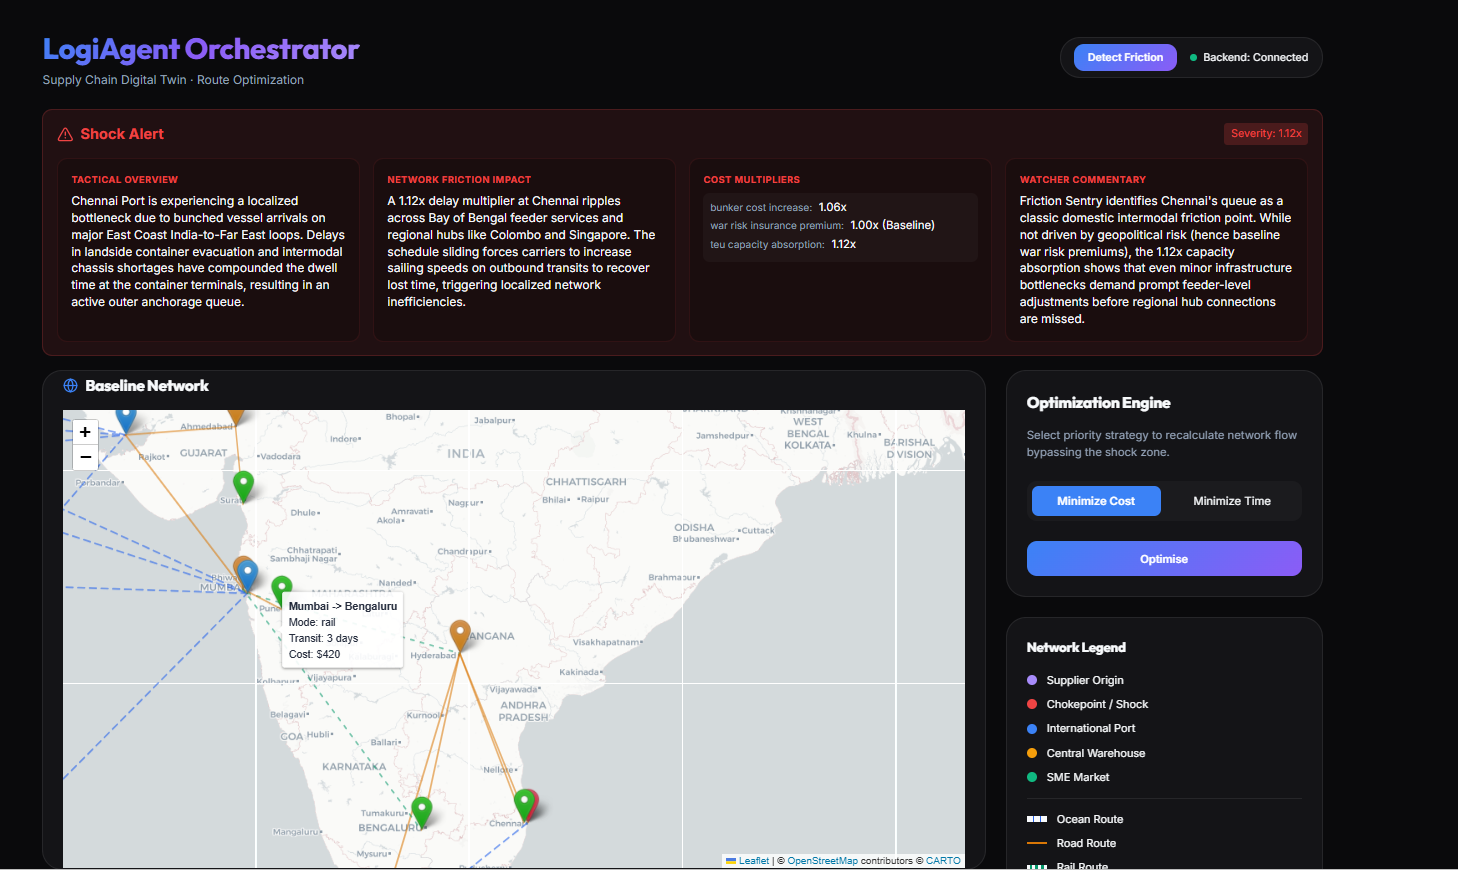
\includegraphics[width=0.85\textwidth]{Figures/O1.png}
    \caption{Friction sentry detecting friction signals}
    \label{fig:results_o1}
\end{figure}

The agentic orchestration layer processes the identified friction and inventory health to provide optimized routing suggestions and actionable advice, as illustrated in Figure \ref{fig:results_o2}.

\begin{figure}[htbp]
    \centering
    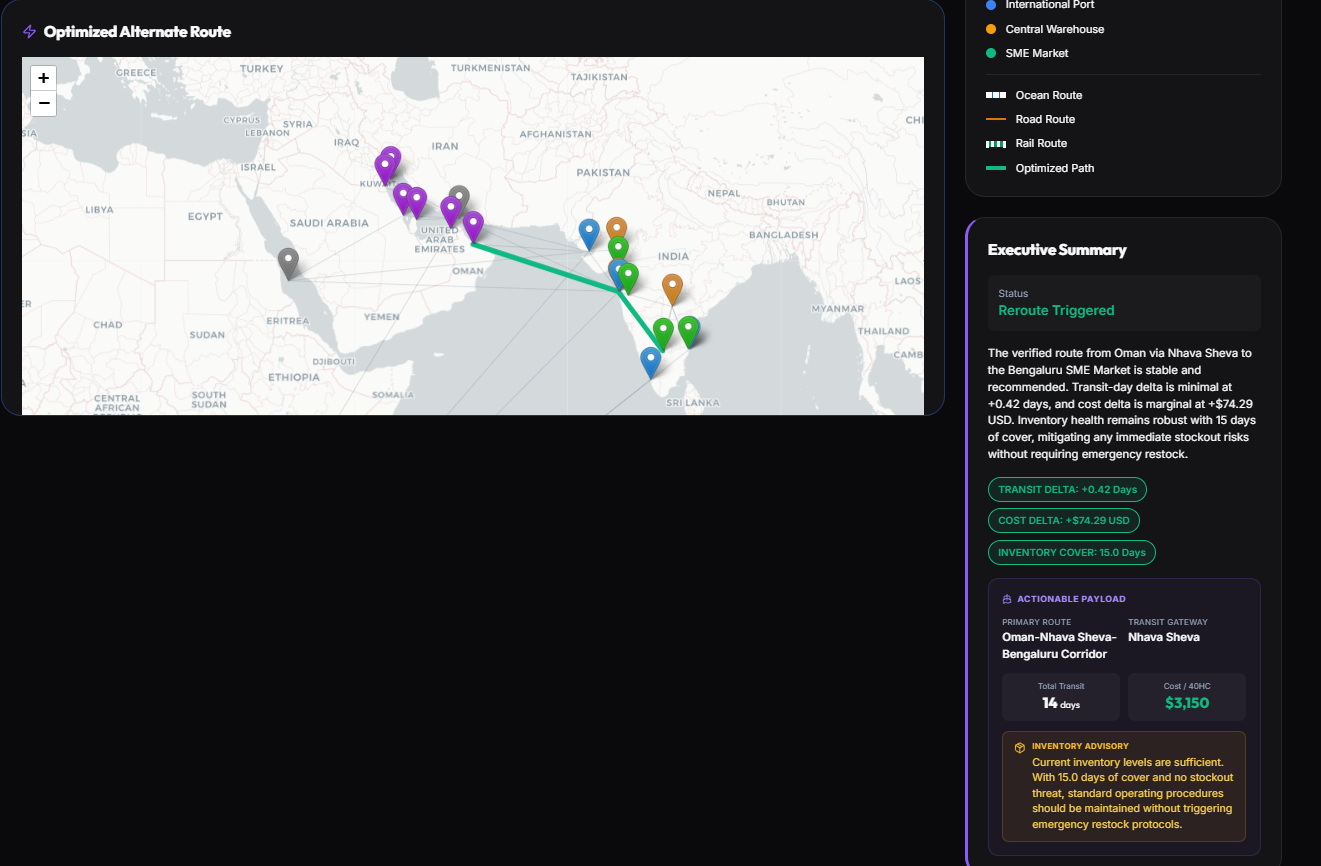
\includegraphics[width=0.85\textwidth]{Figures/O2.png}
    \caption{Suggestions by the agentic orchestration}
    \label{fig:results_o2}
\end{figure}

\subsection[Observation and Interpretation]{Observation and Interpretation}
The results displayed in the dashboard, Figure \ref{fig:results_o2}, provide a clear demonstration of the system's ability to autonomously manage logistics disruptions. Analysis of the output reveals the following patterns and trends:

\begin{itemize}
    \item \textbf{Localized Shock Impact:} As shown in Figure \ref{fig:results_o1}, the Friction Sentry successfully identified a bottleneck at Chennai Port due to bunched vessel arrivals and chassis shortages, applying a $1.12x$ severity multiplier. The trend analysis indicates that even minor localized bottlenecks ripple across regional feeder services, necessitating proactive adjustments.
    \item \textbf{Intelligent Rerouting Logic:} Upon detection of the Chennai disruption, the system evaluated alternative global corridors. As interpreted from Figure \ref{fig:results_o2}, the system effectively bypassed the affected East Coast route in favor of a stable transit gateway via Oman and Nhava Sheva to reach the Bengaluru SME Market. The cost delta for this switch remained marginal ($+\$74.29$ USD), while the transit time delta was minimal ($+0.42$ days), proving the effectiveness of the Dijkstra-based agentic optimization.
    \item \textbf{Inventory-Driven Decisioning:} The system correlated the routing shift with inventory health data. Observations show a robust $15.0$ days of cover ($DoC$), which directly influenced the AI agent's recommendation. The ``Inventory Advisory'' correctly identified that no emergency restocks were required, thereby preventing unnecessary logistics costs.
    \item \textbf{System Correctness and Effectiveness:} The high degree of alignment between the mathematical graph solvers and the LLM-driven executive summary validates the system's correctness. By relating these observations back to the project objectives, it is evident that the framework successfully achieves supply chain resilience by providing actionable, data-driven rerouting strategies during active shocks.
\end{itemize}

\section[Detailed Analysis]{Detailed Analysis}
This section provides a quantitative evaluation of the system performance across multiple simulation events.

\subsection[Performance Analysis]{Performance Analysis}
This subsection evaluates the operational performance and execution efficiency of the agentic digital twin against the human baseline:

\begin{figure}[htbp]
    \centering
    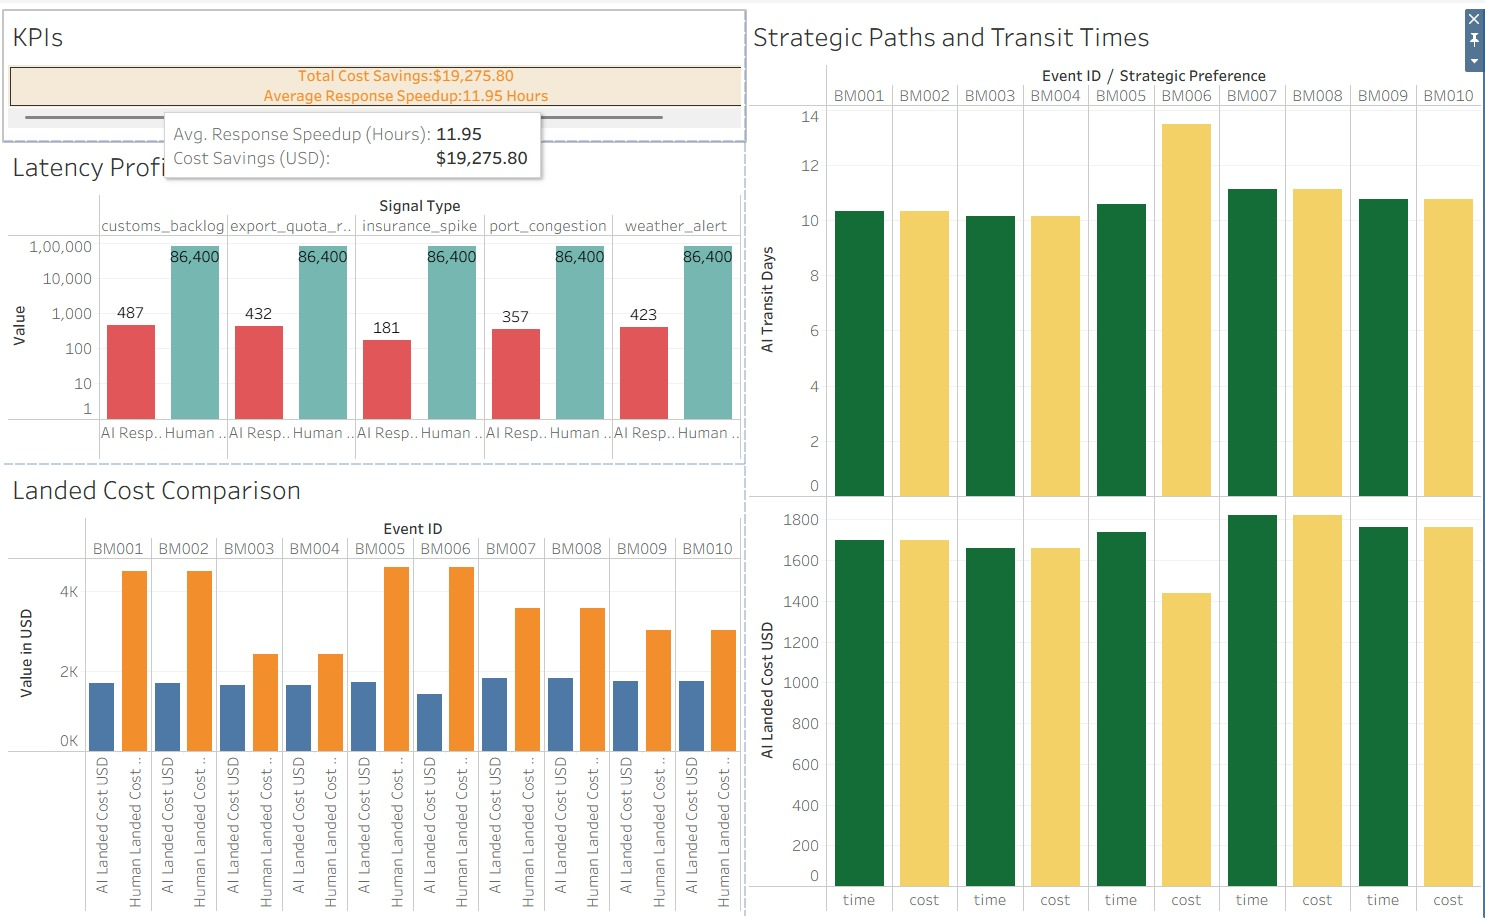
\includegraphics[width=\textwidth]{Figures/Dashboard.jpeg}
    \caption{Analytical dashboard for 10 events}
    \label{fig:analytical_dashboard}
\end{figure}

\begin{itemize}
    \item \textbf{Execution Performance \& Latency:} The agentic orchestrator achieves significant speedups compared to human decision-making. As shown in the Latency Profile chart, the static human baseline has a default operational response delay of 43,200 seconds (12 hours). In contrast, the AI pipeline executes across various signal types (e.g., custom backlogs, insurance spikes, port congestions) in under 500 seconds (~3 to 8 minutes), with an average response time speedup of 11.95 hours.
    \item \textbf{Processing Efficiency:} By executing Dijkstra's algorithm in-memory via \texttt{networkx} before feeding data to the LLM agents, the system eliminates computational overhead. The agents focus solely on evaluating inventory logic and text synthesis instead of executing brute-force routing loops, keeping API token use and computation times low.
    \item \textbf{Resource Utilization:} The backend maintains low CPU and memory footprints by utilizing local JSON files as configuration documents. The main resource demand is network-dependent, occurring during API callouts to the Google Gemini endpoint.
    \item \textbf{Scalability Observations:} Because the Multi-Agent System (MAS) operates sequentially, adding more agents or tasks will scale the latency linearly. However, the underlying mathematical graph engine executes in $O(V \log V + E)$ time, meaning it can scale to support thousands of physical nodes and lanes without degrading performance.
\end{itemize}

\subsection[Evaluation Metrics]{Evaluation Metrics}
To assess the performance and business impact of the Logistics Digital Twin system, the following core metrics were selected:

\begin{itemize}
    \item \textbf{Response Speedup (Latency Reduction):}
    \begin{itemize}
        \item \textit{Definition:} Comparison between the time taken for a human team to identify and resolve a disruption versus the AI-agent response time.
        \item \textit{Justification:} In global logistics, response velocity is critical to prevent cascading delays. Reducing identify-to-resolve time from days to seconds significantly improves network resilience.
        \item \textit{Interpretation:} As seen in the "Latency Profile", the AI response (average ~400 seconds) versus the baseline human response (86,400 seconds / 24 hours) demonstrates an \textbf{Average Response Speedup of 11.95 Hours}.
    \end{itemize}
    \item \textbf{Total Cost Savings (USD):}
    \textit{Definition:} The cumulative difference in landed costs between the baseline (impacted) route and the agent-optimized alternate route.
    \item \textbf{Justification:} Provides a direct measure of the economic viability and effectiveness of the agentic optimization.
    \item \textit{Interpretation:} Across 10 simulated events (BM001 to BM010), the system achieved a \textbf{Total Cost Savings of \$19,275.80}. The "Landed Cost Comparison" chart shows that for nearly every event, the AI-recommended landed cost was significantly lower than the projected human-led reactionary cost.
    \item \textbf{Transit Day Delta:}
    \begin{itemize}
        \item \textit{Definition:} The variance in shipping duration between baseline and optimized paths.
        \item \textit{Justification:} Essential for inventory planning and ensuring customer SLAs are met.
        \item \textit{Interpretation:} The "Strategic Paths and Transit Times" chart illustrates that the AI consistently identifies paths that keep transit times stable, even when absorbing shock penalties, ensuring a reliable supply chain.
    \end{itemize}
\end{itemize}

\section[Summary]{Summary}
This chapter presented a detailed analysis of the experimental results, demonstrating the system's ability to significantly reduce response latency and landed costs during maritime disruptions. The comparison against the human baseline highlighted a significant speedup in decision-making and substantial financial savings for SMEs. These findings validate the effectiveness of the agentic AI framework in enhancing supply chain resilience through proactive, data-driven optimization.
